\documentclass[border=8pt]{standalone}

% --- packages (mirror these in figure.meta.json "requires") ---
\usepackage{tikz}
\usepackage{amsmath}
\usepackage{amssymb}   % \mathbb for $\mathbb{R}$
\usetikzlibrary{positioning, arrows.meta, decorations.pathreplacing, calc}

% --- palette (canonical source: reference/color-palettes/color-palettes.md; light variant) ---
\definecolor{otblue}{HTML}{0072B2}
\definecolor{otorange}{HTML}{E69F00}
\definecolor{otteal}{HTML}{009E73}
\definecolor{otpurple}{HTML}{CC79A7}
\definecolor{otgray}{HTML}{5A5A5A}
\definecolor{otyellow}{HTML}{F0E442}   % Okabe-Ito yellow — activation bars (x, h)

\begin{document}
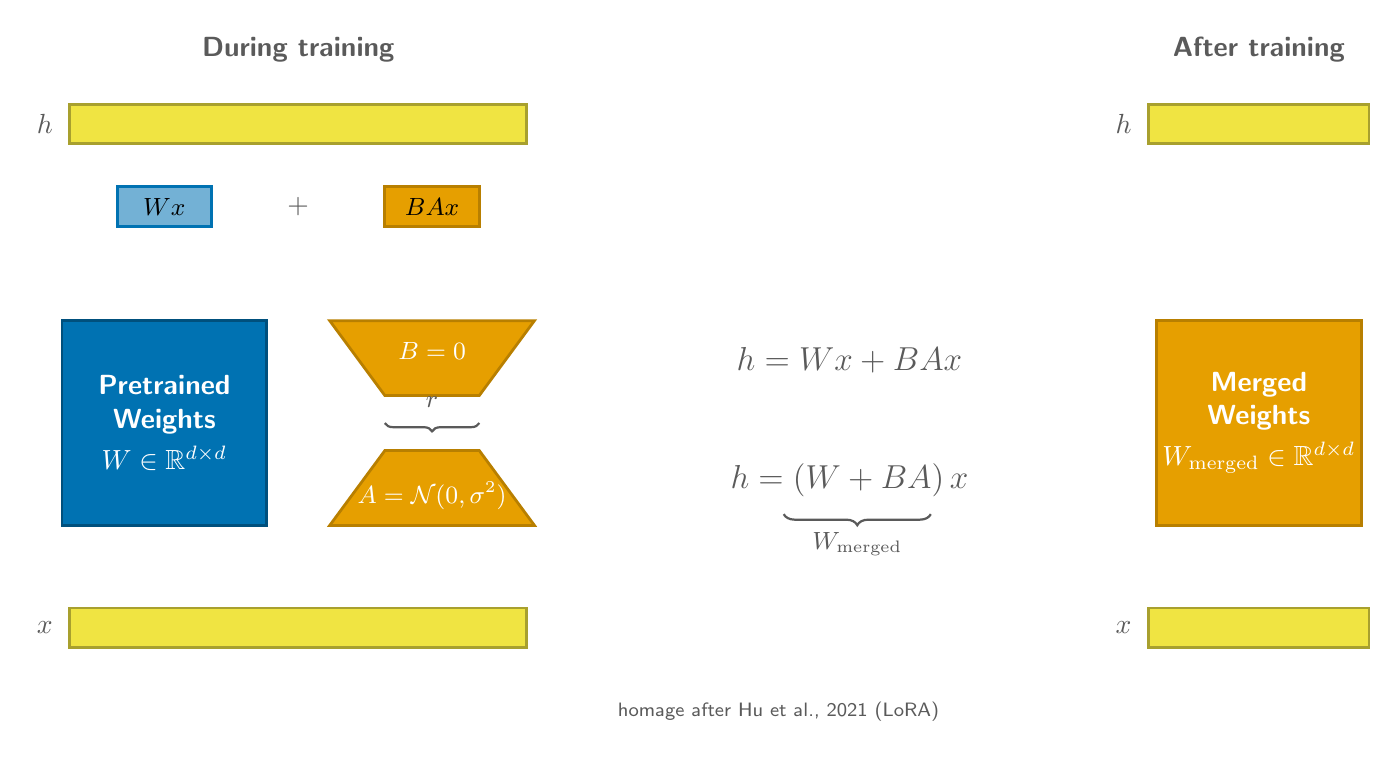
\begin{tikzpicture}[
    >={Stealth[length=2.6mm]},
    font=\sffamily,
    % --- shared element styles -------------------------------------------------
    actbar/.style={                                  % activation bar (x / h): gold, wide & thin
      draw=otyellow!70!black, fill=otyellow, line width=1pt,
      minimum width=58mm, minimum height=5mm, inner sep=0pt},
    actbarC/.style={                                 % narrower gold bar for the single-column zone C
      draw=otyellow!70!black, fill=otyellow, line width=1pt,
      minimum width=28mm, minimum height=5mm, inner sep=0pt},
    bigsq/.style={                                   % dominant solid weight square
      line width=1pt, minimum width=26mm, minimum height=26mm,
      inner sep=0pt, text=white, align=center, font=\sffamily},
    actlabel/.style={font=\sffamily\bfseries, text=otgray},   % the x / h glyphs
    paneltitle/.style={font=\sffamily\bfseries, text=otgray},  % zone titles
    note/.style={font=\sffamily\small, text=otgray},
    midbar/.style={line width=1pt, minimum width=12mm, minimum height=5mm,
      inner sep=0pt, align=center, font=\sffamily\small},
  ]

  % =====================================================================
  % ZONE A — "During training"
  % two parallel columns rising from one shared bottom x bar.
  % =====================================================================
  \def\colL{-1.7}       % left-column centre (blue W square)
  \def\colR{1.7}        % right-column centre (orange B/A bottleneck)
  \def\halfd{1.3}       % half-width at the d-dimension (square/bar half-width)
  \def\halfr{0.6}       % half-width at the rank-r waist (longer short edge)

  % --- bottom input bar x (shared, spans both columns) ---
  \node[actbar] (xbar) at (0,0) {};
  \node[actlabel] at ($(xbar.west)+(-3mm,0)$) {$x$};

  % --- LEFT column: pretrained frozen weights W (solid blue square) ---
  \node[bigsq, draw=otblue!70!black, fill=otblue] (wsq) at (\colL,2.6)
        {\textbf{Pretrained}\\\textbf{Weights}\\[1mm]$W \in \mathbb{R}^{d\times d}$};

  % --- RIGHT column: low-rank update = two orange trapezoids (rank-r bottleneck) ---
  % A: wider at BOTTOM (d) -> narrow at TOP (r)
  \coordinate (Abot) at (\colR, 1.3);
  \coordinate (Atop) at (\colR, 2.25);
  \filldraw[draw=otorange!80!black, fill=otorange, line width=1pt]
    ($(Abot)+(-\halfd,0)$) -- ($(Abot)+(\halfd,0)$)
    -- ($(Atop)+(\halfr,0)$) -- ($(Atop)+(-\halfr,0)$) -- cycle;
  \node[text=white, font=\sffamily\small] (Abox) at ($(Abot)!0.4!(Atop)$)
    {$A = \mathcal{N}(0,\sigma^2)$};
  % B: narrow at BOTTOM (r) -> wider at TOP (d)
  \coordinate (Bbot) at (\colR, 2.95);
  \coordinate (Btop) at (\colR, 3.9);   % top aligned with the Pretrained square top (y=3.9)
  \filldraw[draw=otorange!80!black, fill=otorange, line width=1pt]
    ($(Bbot)+(-\halfr,0)$) -- ($(Bbot)+(\halfr,0)$)
    -- ($(Btop)+(\halfd,0)$) -- ($(Btop)+(-\halfd,0)$) -- cycle;
  \node[text=white, font=\sffamily\small\bfseries] (Bbox) at ($(Bbot)!0.6!(Btop)$)
    {$B = 0$};
  % rank-r brace: HORIZONTAL, spanning the narrow waist (the rank-r dimension),
  % sitting in the gap between A (top) and B (bottom); bump points down onto A.
  \draw[decorate, decoration={brace, mirror, amplitude=3pt}, draw=otgray, line width=0.8pt]
    ($(\colR,2.6)+(-\halfr,0)$) -- ($(\colR,2.6)+(\halfr,0)$)
    node[midway, above=2pt, note] (rbrace) {$r$};

  % --- two mid bars side by side: Wx (sky blue) and BAx (orange) ---
  \node[midbar, draw=otblue, fill=otblue!55] (wxbar) at (\colL,5.35) {$Wx$};
  \node[midbar, draw=otorange!80!black, fill=otorange] (baxbar) at (\colR,5.35) {$BAx$};
  % small gray + joining the two bars (centred between them)
  \node[font=\sffamily\bfseries, text=otgray]
    (plus) at ($(wxbar.east)!0.5!(baxbar.west)$) {$+$};

  % --- output bar h (gold, shared), above the bars ---
  \node[actbar] (hbar) at (0,6.4) {};
  \node[actlabel] at ($(hbar.west)+(-3mm,0)$) {$h$};

  % --- zone title (centered over the panel, above the h bar) ---
  \node[paneltitle, above=4mm of hbar.north] (titleA) {During training};

  % =====================================================================
  % ZONE B — center equations (vertically centred against zone A)
  % =====================================================================
  \coordinate (zoneB) at (7.0, 3.4);   % gap-midpoint between zone A (right edge ~3.0) and zone C (left edge ~10.9)
  \node[text=otgray, font=\large] (eq1) at (zoneB) {$h = Wx + BAx$};
  % second equation: plain (no math \underbrace — its cmex glyphs render as tofu
  % via the dvisvgm DVI route). The brace under "(W + BA)" is drawn as a TikZ
  % brace below, reusing the same decorations.pathreplacing approach as the r brace.
  % single centred node (same x as eq1) so the equation stays in the middle gap
  % and never grows right into zone C. The brace under "(W + BA)" is drawn with
  % relative offsets, reusing the same decorations.pathreplacing approach as r.
  \node[text=otgray, font=\large, below=9mm of eq1]
    (eq2) {$h = (W + BA)\,x$};
  % TikZ brace bracketing the "(W + BA)" subexpression, label W_merged centred below.
  \draw[decorate, decoration={brace, mirror, amplitude=4pt}, draw=otgray, line width=0.8pt]
    ($(eq2.south west)+(8mm,-1mm)$) -- ($(eq2.south east)+(-6mm,-1mm)$)
    node[midway, below=3pt, note] {$W_{\mathrm{merged}}$};

  % =====================================================================
  % ZONE C — "After training" (single bar–square–bar column)
  % =====================================================================
  \def\colC{12.2}
  \node[actbarC] (xbar2) at (\colC,0) {};
  \node[actlabel] at ($(xbar2.west)+(-3mm,0)$) {$x$};
  \node[bigsq, draw=otorange!80!black, fill=otorange] (merged) at (\colC,2.6)
        {\textbf{Merged}\\\textbf{Weights}\\[1mm]$W_{\mathrm{merged}} \in \mathbb{R}^{d\times d}$};
  \node[actbarC] (hbar2) at (\colC,6.4) {};
  \node[actlabel] at ($(hbar2.west)+(-3mm,0)$) {$h$};
  \node[paneltitle, above=4mm of hbar2.north] {After training};

  % =====================================================================
  % provenance caption
  % =====================================================================
  \node[font=\sffamily\scriptsize, text=otgray]
    at ($(xbar.south)!0.5!(xbar2.south)+(0,-8mm)$)
    {homage after Hu et al., 2021 (LoRA)};

\end{tikzpicture}
\end{document}
